\textit{\documentclass[a4paper,12pt]{report}

\usepackage{alltt, fancyvrb, url}
\usepackage{graphicx}
\usepackage[utf8]{inputenc}
\usepackage{float}
\usepackage{hyperref}

% Questo commentalo se vuoi scrivere in inglese.
\usepackage[italian]{babel}
\usepackage[italian]{cleveref}

\title{Relazione\\``Isaccoop''}

\author{Marco Costantini\\Andrea Dotti\\Daniele Pancottini\\Giacomo Pierbattista\\Dilaver Shtini}
\date{\today}

\begin{document}
\maketitle

\tableofcontents

\chapter{Analisi}
Il software mira a realizzare un gioco roguelike liberamente ispirato a ``The Binding Of Isaac". Con ``roguelike" si intende un videogioco tipicamente caratterizzato dall'esplorazione di un dungeon attraverso livelli generati proceduralmente e morte permanente del personaggio giocante.

\section{Requisiti}

\subsection*{Requisiti funzionali obbligatori}
\begin{itemize}
    \item Il protagonista inizierà la partita in una stanza iniziale vuota.
    \\Il giocatore può:
    \begin{itemize}
        \item muoversi liberamente all'interno di ogni stanza e sparare ``sfere di energia''
        \item passare da una stanza all'altra, solo dopo aver sconfitto tutti i \textbf{nemici} che si trovano al suo interno, se presenti
        \item raccogliere monete e cuori (``\textbf{item}'') sparsi nelle varie stanze, se presenti
        \item acquisire una vita raccogliendo i cuori sparsi nelle stanze
        \item comprare potenziamenti (\textbf{powerup}) nell'apposito negozio (\textbf{shop room}), usando le monete raccolte precedentemente
        \item raccogliere un powerup gratis nella stanza \textbf{treasure room}
        \item perdere una vita ogni volta che viene colpito da un nemico o da un proiettile lanciato da esso
        \item visualizzare la struttura del livello giocato nella \textbf{minimappa} per sapere in quale stanza si trova e vedere quali sono state completate
        \item visualizzare le sue (\textbf{``statistiche/caratteristiche"}), ad esempio: il numero di vite rimaste (indicate dai cuori), di monete raccolte, quanto danno riesce a infliggere ai nemici...
        \item il gioco finisce (game over) se il giocatore perde tutte le sue vite/cuori o quando sconfigge tutti i nemici in tutte le stanze, compreso il boss finale
    \end{itemize}
    
    \item Nel gioco vi sono cinque tipi di stanze:
    \begin{itemize}
        \item \textbf{START}: stanza iniziale vuota in cui il giocatore si trova all'inizio della partita
        \item \textbf{TREASURE}: stanza in cui si trova un powerup gratuito, che il giocatore può raccogliere per sconfiggere più facilmente i nemici
        \item \textbf{SHOP}: stanza in cui il giocatore può spendere le monete raccolte precedentemente per comprare altri powerup
        \item \textbf{STANDARD}: stanza in cui si trovano dei nemici e da cui il giocatore può uscire solo dopo averli sconfitti tutti
        \item \textbf{BOSS}: stanza in cui si trova il boss finale; una volta sconfitto, la partita termina.
    \end{itemize}
    \item Una semplice AI (Artificial Intelligence) gestirà i movimenti e gli attacchi dei nemici e del boss finale, i quali cercheranno di colpire il giocatore. Per AI si intende un semplice software che gestisce il movimento e il comportamento dei nemici.
    \item Implementazione della guida/tutorial al gioco, visualizzabile nel menu di gioco prima di iniziare una partita
    \item Gestione della pausa durante il gioco
\end{itemize}

\subsection*{Requisiti funzionali opzionali}
\begin{itemize}
    \item gestione di più livelli, ognuno indipendente dagli altri, con stanze differenti e difficoltà incrementali
    \item gestione del salvataggio a chiusura dell'applicazione per continuare la partita successivamente
    \item effetti sonori
    \item impostazioni di gioco (esempi a titolo indicativo e non esaustivo): \begin{itemize}
        \item scelta del numero minimo e massimo delle stanze che possono formare un livello
        \item numero di livelli da giocare in una partita
    \end{itemize} 
\end{itemize}

\subsection*{Requisiti non funzionali}
\begin{itemize}
    \item il software deve essere portabile, quindi deve essere eseguibile su macchine che eseguono Windows, Mac OS X e Linux/UNIX.
    \item Il software deve garantire un'esperienza di gioco adeguata (fluida, gradevole), indipendentemente dallo stato della partita.
\end{itemize}

\newpage
\section{Analisi e modello del dominio}
Il software permetterà al giocatore di avviare una sessione di gioco, che gestirà l'avanzamento del personaggio principale attraverso le varie stanze che formano il mondo di gioco (\textbf{``livello/level''}).
In un livello sono presenti un numero semicasuale di stanze; in alcune di esse saranno presenti i ``nemici'' da sconfiggere e gli ``item'', mentre in altre si potranno comprare/raccogliere i ``powerup''.
Una volta entrato in una stanza in cui si trovano i nemici, il giocatore dovrà sconfiggerli tutti per poter passare ad un altra stanza.
I nemici saranno gestiti da una semplice AI (come descritto precedentemente) i quali cercheranno di attaccare e uccidere il giocatore. 
Per sconfiggere tali nemici, il giocatore spara le ``sfere di energia''. 
Utilizzando i powerup raccolti o comprati nello shop, il giocatore può sconfiggere più facilmente i nemici. 
Il giocatore perde una vita (indicate con i cuori/``hearts'') ogni volta che viene colpito da un nemico o da un proiettile sparato da esso.
Il gioco terminerà se il giocatore perde tutte le vite.

Le challenge principali di questo progetto sono state:
\begin{itemize}
    \item gestione delle collisioni tra protagonista, item, powerup, nemici e muri delle stanze
    \item creazione dinamica delle stanze con nemici al loro interno
\end{itemize}

\begin{figure}[H]
    \centering{}
    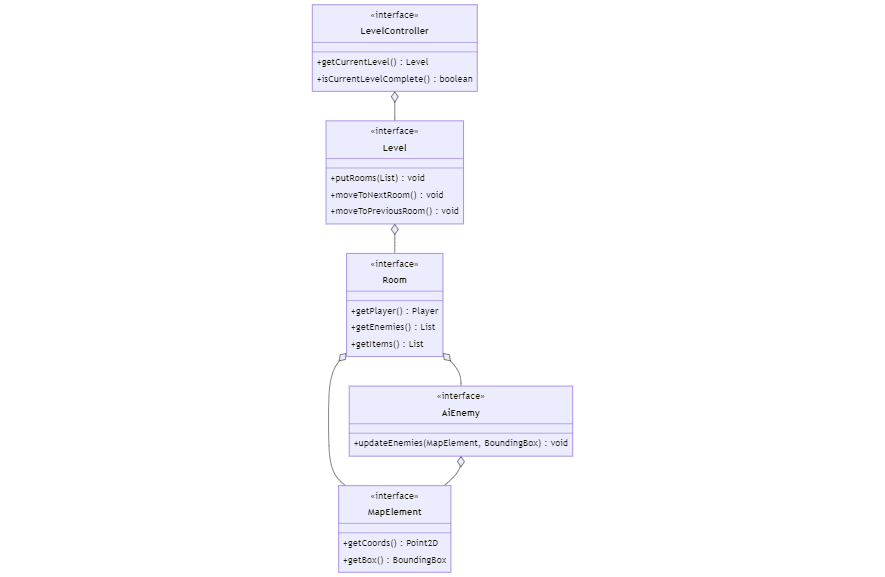
\includegraphics{img/analysis.pdf}
    \caption{Schema UML dell'analisi del problema, con rappresentate le entità principali ed i rapporti fra loro}
    \label{img:analysis}
\end{figure}


\chapter{Design}
\section{Architettura}
Nella progettazione, si è scelto di adottare il pattern architetturale MVC.
\begin{itemize}
    \item \textbf{Model}: ?
    \item \textbf{Controller}: L'interfaccia GameEngine si occupa di gestire {TODO}
    \item \textbf{View}: l'interfaccia Scene.java rappresenta {TODO}, 
        mentre l'interfaccia Graphics si occupa di renderizzare giocatore, nemici, powerup e item sulla mappa di gioco.
\end{itemize}

L'utilizzo di MVC consente di cambiare la tecnologia alla base della View senza modificare 
né Model né Controller del software:
infatti sarà necessario cambiare l'implementazione dei file SwingScene, SwingGraphics e degli altri file
che contengono l'implementazione delle altre GUI realizzate, utilizzando la nuova tecnologia, 
sostituendo così l'implementazione attuale basata sul framework Swing con la nuova tecnologia scelta.


\begin{figure}[h]
    \centering{}
    \includegraphics[width=\textwidth]{img/arch}
    \caption{Schema UML architetturale di GLaDOS. L'interfaccia \texttt{GLaDOS} è il controller del sistema, mentre \texttt{Input} ed \texttt{Output} sono le interfacce che mappano la view (o, più correttamente in questo specifico esempio, il boundary). Un'eventuale interfaccia grafica interattiva dovrà implementarle entrambe.}
    \label{img:goodarch}
\end{figure}


In \Cref{img:goodarch} è esemplificato il diagramma UML architetturale.


\section{Design dettagliato}

\subsection*{Marco Costantini}
{TODO}

\subsection*{Andrea Dotti}

\paragraph{Problema} Occorre un ``controller" per l'utente in modo da interagire con il programma (ad esempio per muovere il player). 
\paragraph{Soluzione} La linea guida per soluzione che abbiamo deciso di seguire prende spunto dal pattern mostratoci dal professor. Ricci: \url{https://github.com/aricci303/game-as-a-lab/tree/master/Game-As-A-Lab-Step-7-mosquito-AI/src/rollball/input}. Questa parte del progetto era una dei tre fondamenti del pattern MVC, ovvero la logica di aggiornamento dall'esterno (in-put) della parte del model. Ho creato una interfaccia InputController con i metodi per controllare le quattro direzioni. La KeyboardInputController implementa l'interfaccia precedentemente descritta e la estende con due metodi per aggiornare la premuta / il rilascio dei tasti che definiscono le direzioni. Ho deciso di creare questa classe sufficientemente generica in modo che potesse essere usata per l'input da tastiera sia del movimento che per sparare i proiettili. Successivamente ho creato l'interfaccia dell'InputComponent con il metodo update, il quale viene in seguito implementato dalle due sottoclassi PlayerInputComponent e ShotInputComponent. Questo metodo è molto importante perché va effettivamente a legare l'input dall'InputController al model. Infatti le sottoclassi implementano rispettivamente il loro update che effettua azioni differenti in base alle informazioni che arrivano dal controller. Il Player contiene nei sui campi i due controller, per il movimento e per lo sparo.
\begin{figure}[H]
    \centering{}
    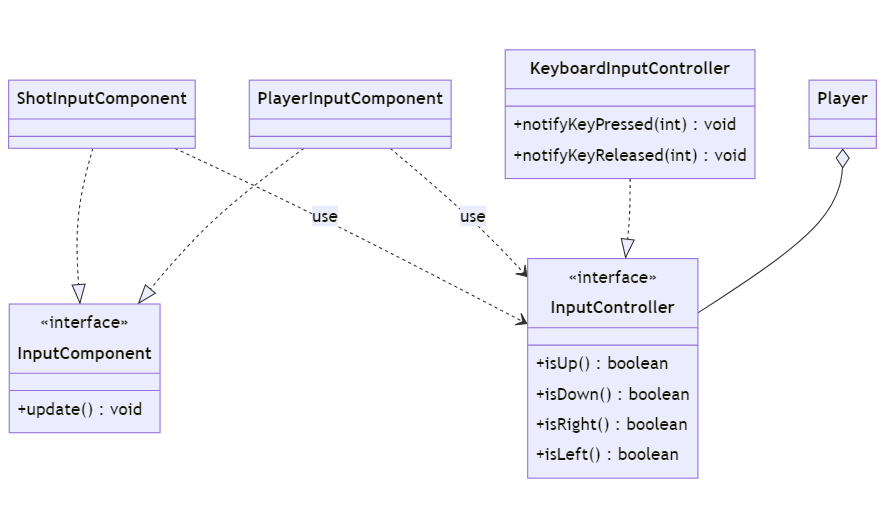
\includegraphics[scale=0.4]{diagram/InputComponent.png}
    \caption{Rappresentazione UML della parte di Controller del pattern MVC}
    \label{img:InputComponent}
\end{figure}

\paragraph{Problema} Occorre un altro ``controller" all'utente per cambiare stanza e per mettere in pausa il gioco. 
\paragraph{Soluzione} Analogamente al pattern seguito in precenza ho creato un nuovo controller, che si differenzia dal precedente per il tipo di notifica di cui deve tenere traccia anche se il principio di design rimane lo stesso. Qui ad esempio le azioni non sono continuative, ma si potrebbero definire atomiche perché avvengono istantaneamente se le condizioni richieste in seguito nella parte che fa da ponte tra controller e model (ActionComponent) sono soddisfatte.
\begin{figure}[H]
    \centering{}
    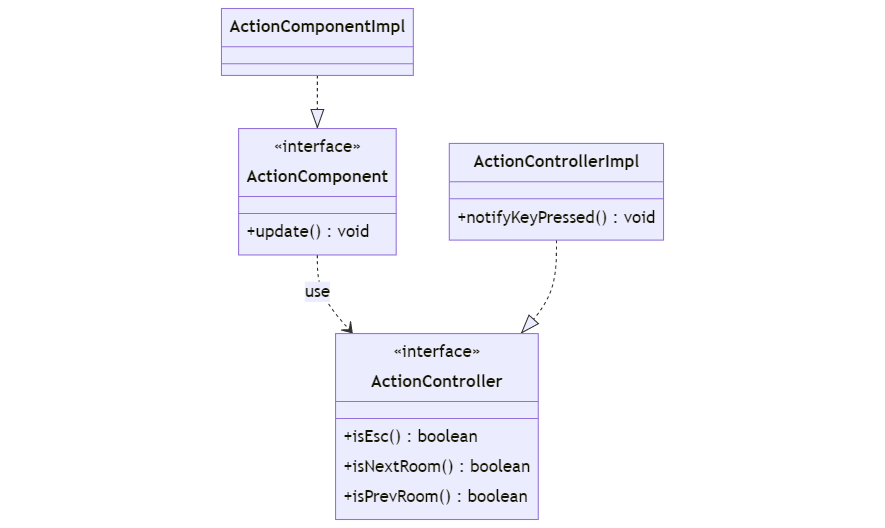
\includegraphics[scale=0.4]{diagram/ActionComponent.png}
    \caption{Rappresentazione UML della parte di ActionController}
    \label{img:ActionComponent}
\end{figure}

\paragraph{Problema} Occorre schierare diversi tipi di elementi (es. enemy, boss, items ecc.) all'interno di una stanza, in modo casuale o ordinato in base al tipo di stanza.
\paragraph{Soluzione} Ho sfruttato la generalizzazione di MapElemet che viene esteso da tutti gli elementi del gioco, in modo che a prescindere dal tipo di elemento si possa andare a settare le sue coordinate all'interno di una stanza di cui vengono passate le dimensioni come parametri del metodo ``setPosition". Dall'interfaccia Spawn ne implemento due sottoclassi diverse (specializzazione), una per gli elementi che devono essere schierati in modo ordinato e una per quello casuale. Sarà poi la Room che dopo aver creato gli elementi chiamerà il metodo della sottoclasse che le serve. Per esempio una ShopRoom e una TreasureRoom andranno a chiamare il metodo dalla classe SpawnOrdered, mentre la stanza di nemici normale andrà chiamare il metodo dalla classe SpawnRandom.

\begin{figure}[H]
    \centering{}
    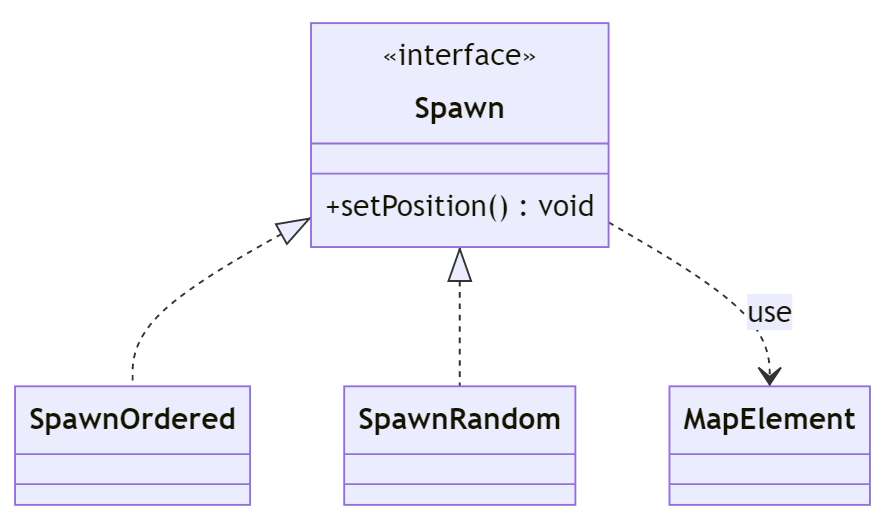
\includegraphics[scale=0.4]{diagram/Spawn.png}
    \caption{Rappresentazione UML per lo schieramento di MapElemnt dentro la stanza}
    \label{img:Spawn}
\end{figure}

\paragraph{Problema} Occorre effettuare l'acquisto dei PowerUp da parte del Player, controllando che quest'ultimo abbia abbastanza monete e nel caso affermativo applicare il PowerUp al Player.
\paragraph{Soluzione} In questo caso ho creato una interfaccia Shop che definisce il metodo ``buyItem", il quale ha come parametri il Player e un PowerUp. La classe ShopImpl implementa questo metodo andando a controllare la quantità delle monete del player con il costo del PowerUp. Nel caso il Player abbia abbastanza monete avviene l'aquisto andando a rimuovere dalle monete del Player il prezzo del PowerUp e in seguito esegue il metodo ``interact" del PowerUp che applica al Player il potenziamento.
\begin{figure}[H]
    \centering{}
    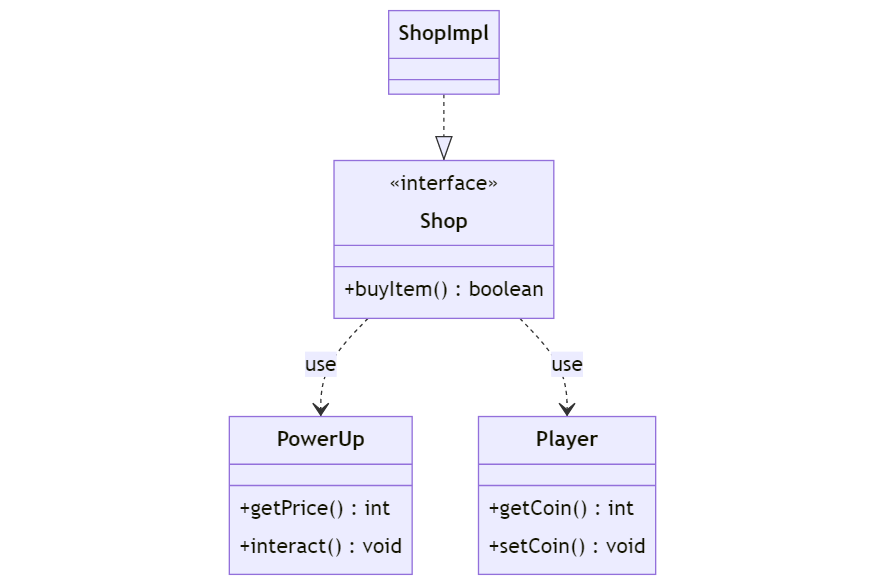
\includegraphics[scale=0.4]{diagram/Shop.png}
    \caption{Rappresentazione UML per la funzione di acquisto dei PowerUp da parte del Player}
    \label{img:Shop}
\end{figure}

\paragraph{Problema} Occorre effettuare un controllo per capire se avviene una collisione tra due oggetti in uno spazio bidimensionale.
\paragraph{Soluzione} Per risolvere questo problema abbiamo visionato il progetto del professore Ricci: \url{https://github.com/aricci303/game-as-a-lab/blob/master/Game-As-A-Lab-Step-7-mosquito-AI/src/rollball/model/BoundingBox.java}, rifattorizzandolo in modo oppurtuno. Ho implementato l'interfaccia BoundingBox in due sottoclassi (RectBoundingBox e CircleBoundingBox) che si differenziano per la forma del BoundingBox, uno circolare e uni rettangolare. Entrambi ereditano i metodi isCollidingWithCricle e isCollidingWithRecPerimeter che ovviamente vengono implementati in modo diverso a seconda della sottoclasse.
\begin{figure}[H]
    \centering{}
    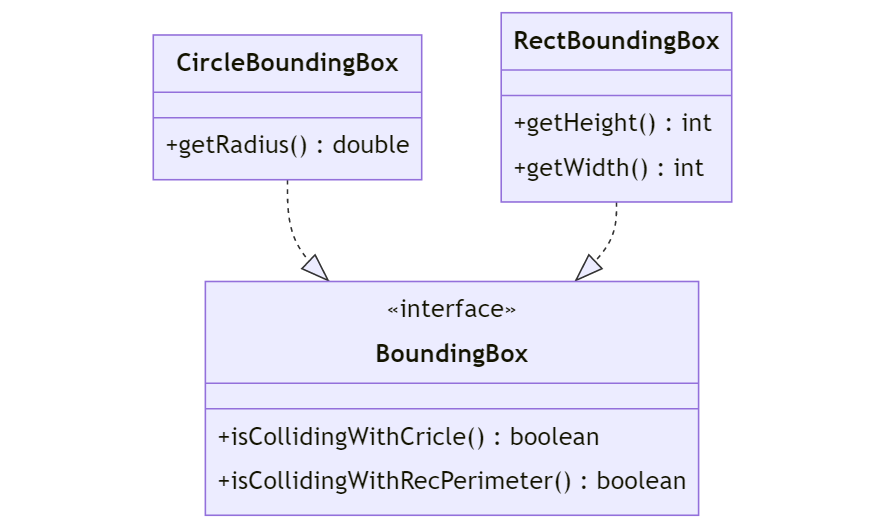
\includegraphics[scale=0.4]{diagram/BoundingBox.png}
    \caption{Rappresentazione UML del controllo collisioni tra due BoundingBox}
    \label{img:BoundingBox}
\end{figure}

\subsection*{Daniele Pancottini}
{TODO}


\subsection*{Giacomo Pierbattista}

\paragraph{Problema} Occorre creare una stanza rispettando certi requisiti
\paragraph{Soluzione} Come descritto nella sezione ``requisiti funzionali'', in questo gioco sono previsti 5 tipi
di stanza, ognuno con le sue caratteristiche. 
\\Ho utilizzato il pattern Builder per creare le stanze ``a basso livello'', nel senso che la classe RoomBuilder (insieme alla classe di utility RoomBuilderUtils) si è occupata di creare fisicamente la stanza, nascondendo la logica dietro la creazione della stanza stessa. 
In questo modo, le altre classi non hanno bisogno di sapere come deve essere costruita una stanza. 
RoomBuilder crea un stanza usando il cosiddetto ``fluent style'' \footnote{\url{https://en.wikipedia.org/wiki/Fluent_interface}}: 
per costruire una stanza è necessario innanzitutto chiamare i metodi obbligatori (necessari per tutti i tipi di stanza); successivamente, a seconda della stanza da creare, devono essere chiamati gli altri metodi
che si occuperanno di impostare le caratteristiche rimanenti.
Chiamando il metodo \texttt{build()} la stanza verrà effettivamente
creata solo se la configurazione è corretta.
\\Il pattern Builder, quindi, porta alcuni vantaggi:
\begin{itemize}
    \item non vengono mai create stanze mal configurate 
    \item nasconde la logica dietro la creazione della stanza stessa
    \item è possibile cambiare la configurazione della stanza (e i relativi controlli).
\end{itemize}
\begin{figure}[H]
    \centering{}
    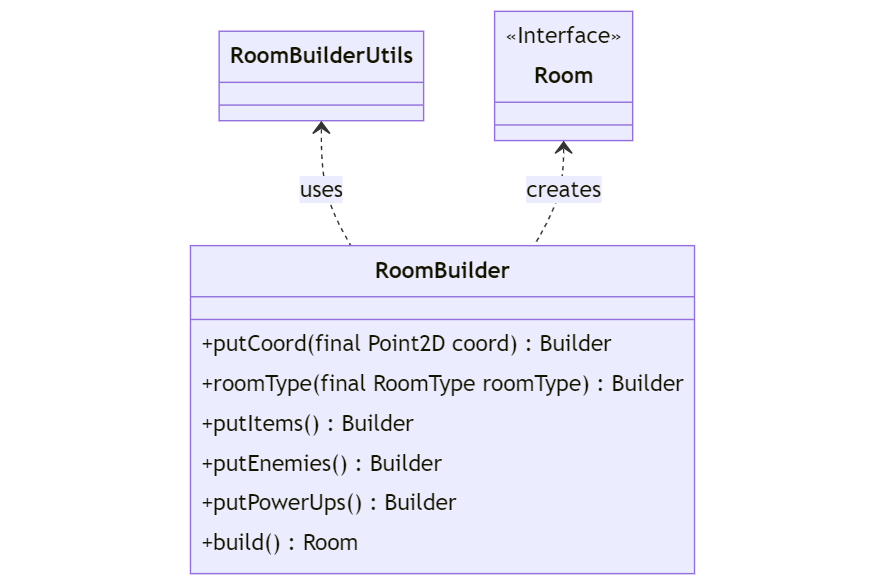
\includegraphics[scale=0.5]{diagram/roombuilder.png}
    \caption{Rappresentazione UML del pattern Builder per la creazione delle stanze a ``basso livello''}
    \label{img:roomBuilder}
\end{figure}

\paragraph{Problema} Occorre creare un numero random di stanze, ognuna con le sue caratteristiche, nascondendone la logica.
\paragraph{Soluzione} Nel punto precedente, RoomBuilder crea le stanze a ``basso livello''; occorre qualcosa che permetta di istanziarle ad ``alto livello'', incapsulando la procedura di creazione delle stesse. 
\\Ho utilizzato il pattern Factory Method: l'interfaccia RoomFactory offre un metodo
per creare ogni tipo di stanza (\texttt{buildStartRoom(), buildStandardRoom()...}),
più un metodo ``intelligente'' \texttt{buildRoomInProperOrder()}, che crea una stanza del tipo appropriato ogni volta che viene chiamato.
\\RoomFactory, per creare le stanze, si appoggia a RoomBuilder precedentemente descritto: in RoomFactory è incapsulata la procedura per la creazione delle stanze, 
mentre RoomBuilder si limita a creare le stanze, seguendo le indicazioni contenute in RoomFactory.

\begin{figure}[H]
    \centering{}
    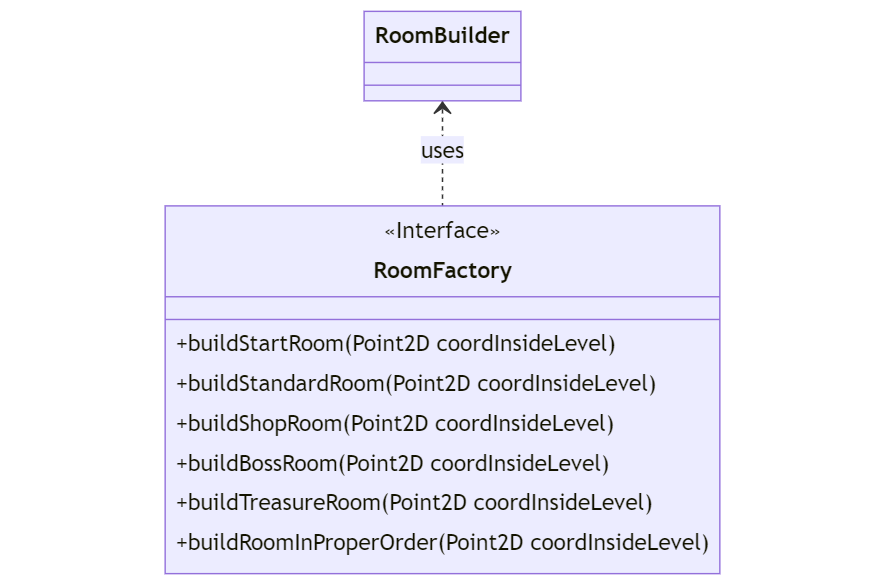
\includegraphics[scale=0.5]{diagram/roomFactory.png}
    \caption{Rappresentazione UML del pattern Factory Method per la creazione delle stanze ad ``alto livello''}
    \label{img:roomFactory}
\end{figure}


\subsubsection{Creazione delle stanze}
\paragraph{Problema} Le stanze hanno bisogno di una coordinata all'interno del livello.
\paragraph{Soluzione} Poiché tutte le entità del gioco (nemici, powerup e item) hanno una coordinata,
è stata creata l'interfaccia MapElement, che permette di avere un getter e un setter per la coordinata. 
L'interfaccia Room estende MapElement, in modo tale che le entità di cui sopra e 
le stanze abbiano lo stesso metodo per accedere e settare la coordinata, evitando
così inutili ripetizioni codice e rispettando il principio DRY - Don't Repeat Yourself.
\begin{figure}[H]
    \centering{}
    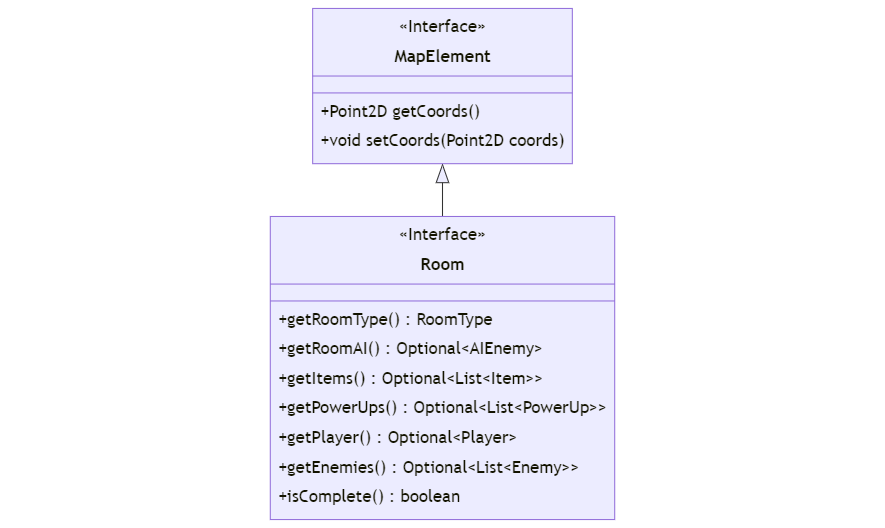
\includegraphics[scale=0.5]{diagram/mapelement.png}
    \caption{Rappresentazione UML dell'interfaccia Room che estende l'interfaccia MapElement, per ereditarne i metodi evitando ripetizioni}
    \label{img:mapelement}
\end{figure}


\subsubsection{Creazione del mondo di gioco (livello/level)}
\paragraph{Problema} E' necessario creare il livello in modo dinamico, nascondendone
la logica.
\paragraph{Soluzione} Anche in questo caso ho utilizzato il pattern Factory Method.
Infatti, LevelFactory si occupa di creare un livello attraverso il 
metodo \texttt{createLevel()}, ma internamente usa il metodo \texttt{buildRoomInProperOrder()} di RoomFactory per creare le stanze richieste, il quale, a sua volta, si occuperà di costruire e restituire la stanza appropriata.
In questo modo, anche il livello viene creato senza che le altri classi si preoccupino di come farlo effetivamente.

\begin{figure}[H]
    \centering{}
    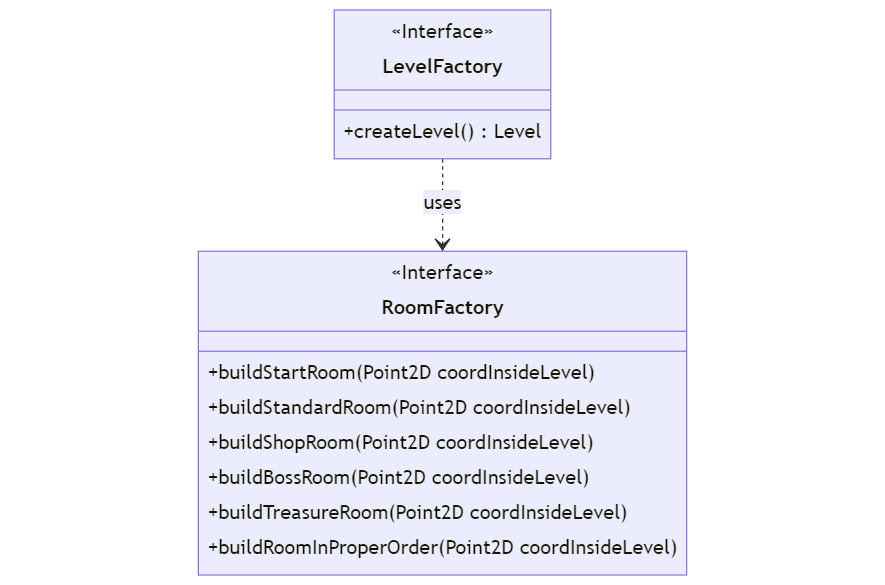
\includegraphics[scale=0.5]{diagram/levelFactory.png}
    \caption{Rappresentazione UML del pattern Factory Method per la creazione dei livelli}
    \label{img:levelFactory}
\end{figure}

\subsubsection{Gestione di un livello}
\paragraph{Problema} Gestire lo stato di un livello
\paragraph{Soluzione} La stanza è l'unità fondamentale di gioco: tutto si svolge al suo interno. Nel mondo di gioco esistono più stanze: le stanze nel loro insieme costituiscono il ``livello''. 
\\Il livello gestisce il suo stato interno (cioè riesce a determinare in quale stanza si trova il giocatore, se una certa stanza è completa, se tutto il livello è completo).
\footnote{Una stanza è completa se non sono rimasti nemici da sconfiggere; \\un livello è completo se tutte le stanze che lo compongono sono complete.}

\begin{figure}[H]
    \centering{}
    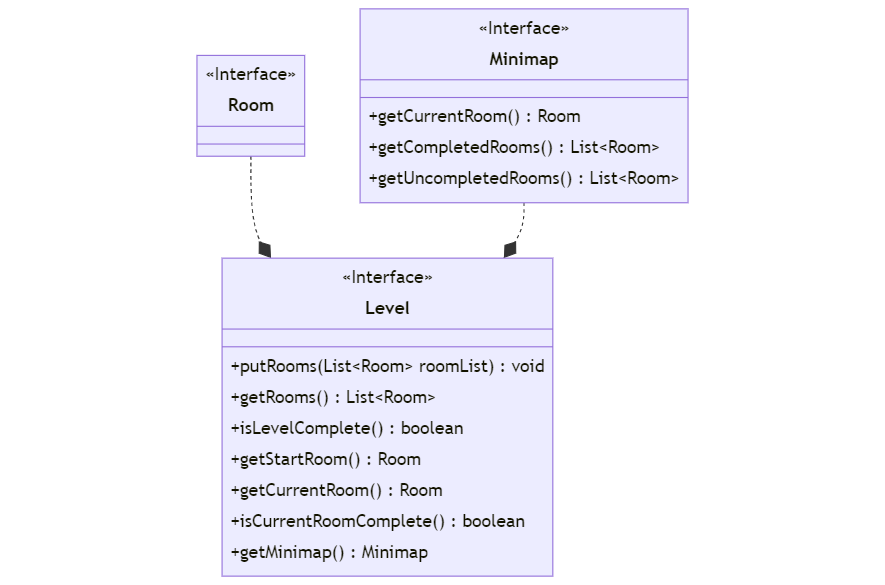
\includegraphics[scale=0.5]{diagram/minimapLevel.png}
    \caption{Rappresentazione UML del }
    \label{img:minimapLevel}
\end{figure}

\subsubsection{Gestione di più livelli}
\paragraph{Problema} Gestire più livelli dinamicamente
\paragraph{Soluzione} Come descritto precedentemente, un singolo livello riesce a 
gestire il suo stato. 
Ho progettato l'interfaccia LevelController pensando di generalizzare il più possibile: un LevelController, infatti, può gestire più livelli, che idealmente vengono giocati uno dopo l'altro.
Questa funzionalità, però, non è stata implementata completamente in quanto era
prevista come requisito opzionale, e per mancanza di tempo non è stata inserita
effettivamente nel gioco.
Un LevelController si occupa di creare uno o più livelli, a seconda della configurazione interna, utilizzando la LevelFactory: anche in questo caso ho
delegato la creazione di un oggetto a una classe/interfaccia apposita.

\begin{figure}[H]
    \centering{}
    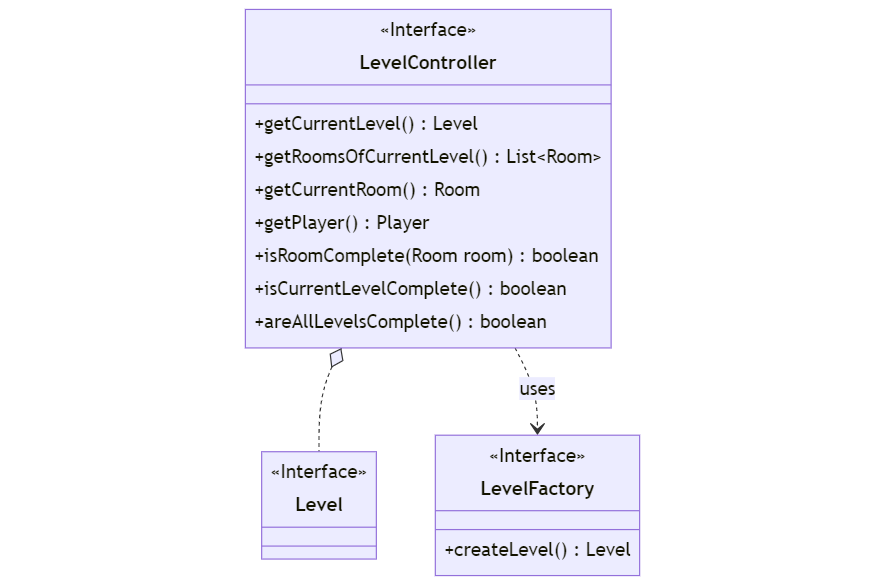
\includegraphics[scale=0.5]{diagram/levelController.png}
    \caption{Rappresentazione UML del }
    \label{img:levelController}
\end{figure}

\subsection*{Dilaver Shtini}
\subsubsection{Creazione e gestione del Player}
\paragraph{Problema}
Il concetto di sparo è in comune anche con i nemici e il boss, quindi, non può essere specifico solo per il player, deve essere generico, inoltre il movimento deve essere gestito diversamente da quello dei nemici.
\paragraph{Soluzione}
Per lo sparo viene utilizzato il pattern “Strategy” dove viene creata un’interfaccia funzionale con il metodo “hit” e due sottoclassi che la implementano, “NonshootingHitStrategy” e “ShootingHitStrategy”, così da poter essere utilizzato sia dal player, il quale userà lo “ShootingHitStrategy”, che dai nemici, che sono di tue tipi, e dal boss, che, come il player, utilizzerà lo “ShootingHitStrategy”.                          Per il movimento invece viene creata un’interfaccia “MapElement”, che viene usata da tutti gli elementi che hanno una posizione nella mappa, per gestire le coordinate, che viene implementata da una classe astratta “AbstractMapElement”, la quale aggiunge il raggio e il boundingBox, estesa dal player.
\newpage
\begin{figure}
    \centering{}
    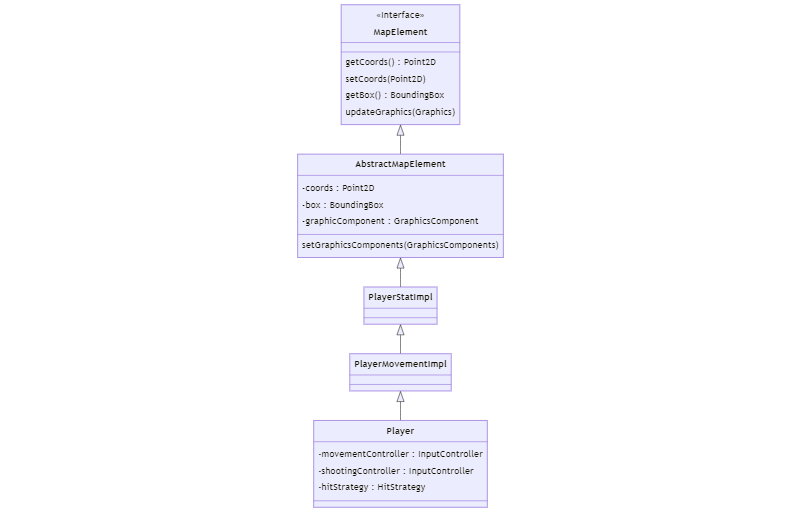
\includegraphics[scale=0.5]{diagram/player.png}
    \caption{Creazione del player}
    \label{player}
\end{figure}
\begin{figure}
    \centering{}
    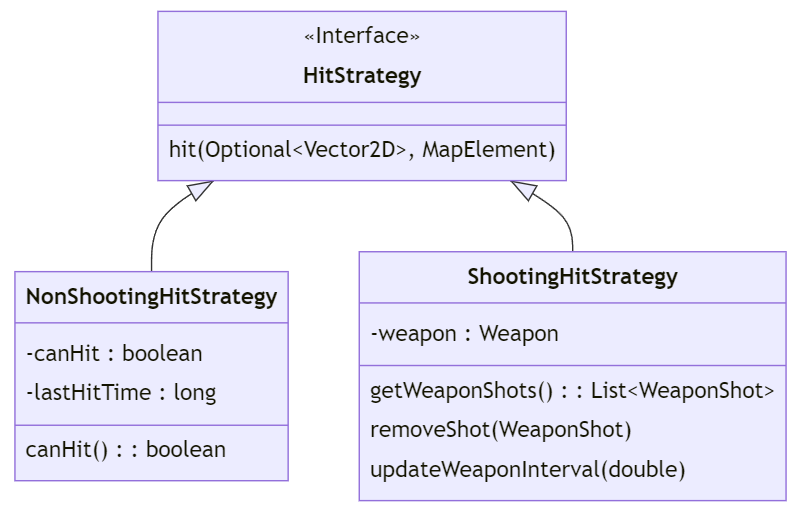
\includegraphics[scale=0.5]{diagram/hitStrategy.png}
    \caption{Pattern strategy per il colpo}
    \label{player}
\end{figure}
\newpage
\subsubsection{Creazione e gestione del Boss}
\paragraph{Problema}
Gestire il cambio del tipo di movimento e lo sparo.
\paragraph{Soluzione}
Per il movimento dei nemici, quindi anche del Boss, viene utilizzato il pattern “Strategy” creando un’interfaccia funzionale con il metodo “move”, implementata poi dai due tipi di movimento: “NonShootingMovementStrategy” e “ShootingMovementStrategy”, che prende in ingresso la posizione attuale del nemico e la posizione del player, ovvero la posizione verso cui andrà il nemico nella modalità “NonShootingMovementStrategy”. Nel Boss, inoltre, si crea una mappa per gestire i due tipi di movimento e un metodo, “changeMode”, che si appresta al cambio del tipo ogni n secondi. Per lo sparo invece, simile al Player, si crea la strategia di tipo “ShootingHitStrategy”.
\begin{figure}
    \centering{}
    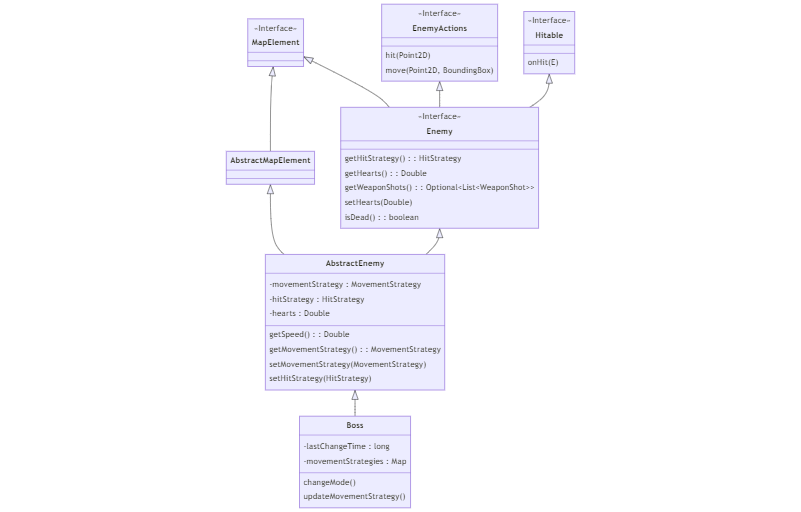
\includegraphics[scale=0.5]{diagram/boss.png}
    \caption{Creazione del boss}
    \label{Boss}
\end{figure}
\begin{figure}
    \centering{}
    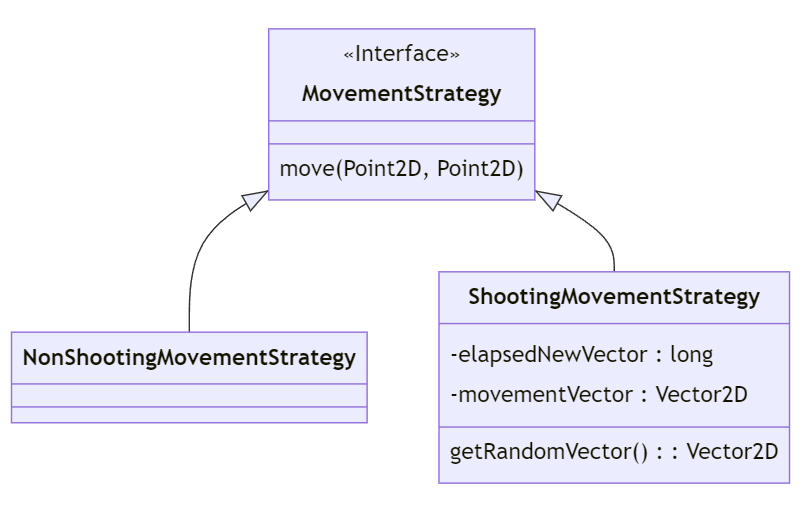
\includegraphics[scale=0.5]{diagram/movementStrategy.png}
    \caption{Pattern strategy per il movimento}
    \label{Boss}
\end{figure}

\subsection*{Esempio minimale (e quindi parziale) di sezione di progetto con UML ben realizzati}

\subsubsection{Personalità intercambiabili}

\begin{figure}[H]
    \centering{}
    \includegraphics[width=\textwidth]{img/strategy}
    \caption{Rappresentazione UML del pattern Strategy per la personalità di GLaDOS}
    \label{img:strategy}
\end{figure}

\paragraph{Problema} GLaDOS ha più personalità intercambiabili, la cui presenza deve essere trasparente al client.

\paragraph{Soluzione} Il sistema per la gestione della personalità utilizza il \textit{pattern Strategy}, come da
\Cref{img:strategy}: le implementazioni di \texttt{Personality} possono essere modificate, e la
modifica impatta direttamente sul comportamento di GLaDOS.

\subsubsection{Riuso del codice delle personalità}

\begin{figure}[H]
    \centering{}
    \includegraphics[width=\textwidth]{img/template}
    \caption{Rappresentazione UML dell'applicazione del pattern Template Method alla gerarchia delle Personalità}
    \label{img:template}
\end{figure}

\paragraph{Problema} In fase di sviluppo, sono state sviluppate due personalità, una buona ed una cattiva.
Quella buona restituisce sempre una torta vera, mentre quella cattiva restituisce sempre la
promessa di una torta che verrà in realtà disattesa.
Ci si è accorti che diverse personalità condividevano molto del comportamento,
portando a classi molto simili e a duplicazione.

\paragraph{Soluzione} Dato che le due personalità differiscono solo per il comportamento da effettuarsi in caso di percorso completato con successo,
è stato utilizzato il \textit{pattern template method} per massimizzare il riuso, come da \Cref{img:template}.
Il metodo template è \texttt{onSuccess()}, che chiama un metodo astratto e protetto
\texttt{makeCake()}.

\subsubsection{Gestione di output multipli}

\begin{figure}[H]
    \centering{}
    \includegraphics[width=.7\textwidth]{img/observer}
    \caption{Il pattern Observer è usato per consentire a GLaDOS di informare tutti i sistemi di output in ascolto}
    \label{img:observer}
\end{figure}

\paragraph{Problema} Il sistema deve supportare output multipli. In particolare, si richiede che vi sia un logger che stampa a terminale o su file,
e un'interfaccia grafica che mostri una rappresentazione grafica del sistema.

\paragraph{Soluzione} Dato che i due sistemi di reporting utilizzano le medesime informazioni, si è deciso di raggrupparli dietro l'interfaccia \texttt{Output}.
A questo punto, le due possibilità erano quelle di far sì che \texttt{GLaDOS} potesse pilotarle entrambe.
Invece di fare un sistema in cui questi output sono obbligatori e connessi, si è deciso di usare maggior flessibilità (anche in vista di future estensioni)
e di adottare una comunicazione uno-a-molti fra \texttt{GLaDOS} ed i sistemi di output.
La scelta è quindi ricaduta sul \textit{pattern Observer}: \texttt{GLaDOS} è observable, e le istanze di \texttt{Output} sono observer.
%
Il suo utilizzo è esemplificato in \Cref{img:observer}




\begin{figure}[h]
    \centering{}
    \includegraphics[width=\textwidth]{img/badarch}
    \caption{Schema UML mal fatto e con una pessima descrizione, che non aiuta a capire. Don't try this at home.}
    \label{img:badarch}
\end{figure}


\chapter{Sviluppo}
\section{Testing automatizzato}
Sono state realizzate diverse classi di test automatizzato, utilizzando JUnit 5.
Non sono stati realizzati test automatici sulla GUI per mancanza di tempo.
I test sono stati realizzati secondo quanto segue:
\subsection*{Marco Costantini}
\begin{itemize}
    \item TestItem
\end{itemize}
\subsection*{Andrea Dotti}
\begin{itemize}
    \item TestShop
\end{itemize}
\subsection*{Daniele Pancottini}
\begin{itemize}
    \item TestEnemy
\end{itemize}
\subsection*{Giacomo Pierbattista}
Ognuno dei seguenti file contiene un test per ogni metodo delle rispettive interfacce, in modo da verificare
il corretto funzionamento di ogni singolo metodo.
\begin{itemize}
    \item LevelControllerTest
    \item LevelFactoryTest
    \item LevelTest
    \item RoomBuilderTest
    \item RoomFactoryTest
    \item RoomTest
\end{itemize}

\subsection*{Dilaver Shtini}
\begin{itemize}
    \item TestPlayer
\end{itemize}



\section{Metodologia di lavoro}
Il lavoro è stato diviso tra i componenti del gruppo all'inizio, in modo da permettere a tutti di 
lavorare indipendentemente dagli altri il più possibile.
E' stato necessario riunirsi per discutere sull'implementazione e/o sulla dichiarazione di interfacce e 
classi comuni.

Abbiamo utilizzato lo strumento di version control \textbf{Git} per poter sviluppare 
il software in modo più agevole.
\\Il branch principale è stato denominato \textit{master}.
Dal \textit{master} sono stati creati vari branch, chiamati ``feature-featureName''; 
ognuno di essi identificava la feature che doveva essere implementata. 
La divisione delle feature tra i vari componenti del gruppo è stata tale da permettere 
a ognuno di lavorare nel proprio branch indipendentemente dagli altri.
\\Abbiamo lavorato in modo tale che tutte le modifiche venissero apportate nei vari branch 
``feature-featureName''; solo dopo aver testato che tutto funzionasse correttamente, 
tali modifiche sono state unite sul branch \textit{master}.
\\In questo modo, il software contenuto nel branch \textit{master} funzionava sempre correttamente.


\subsection*{Marco Costantini}
In autonomia, ho sviluppato
\begin{itemize}
    \item \begin{verbatim}it.unibo.isaccoop.core.* \end{verbatim} esclusa la funzione di pausa in GameLoopImpl.java
    \item \begin{verbatim}it.unibo.isaccoop.model.item.* \end{verbatim}
    \item \begin{verbatim}it.unibo.isaccoop.model.powerup.* \end{verbatim}
\end{itemize}
Ho sviluppato: 
\begin{itemize}
    \item in collaborazione con Daniele Pancottini: 
        \begin{itemize}
        \item \begin{verbatim}it.unibo.isaccoop.model.creator.* \end{verbatim} 
        \item \begin{verbatim}it.unibo.isaccoop.graphics.factory.* \end{verbatim}
    \end{itemize}
    \item in collaborazione con Daniele Pancottini e Andrea Dotti \item \begin{verbatim}it.unibo.isaccoop.model.collision.* \end{verbatim}
\end{itemize} 

\subsection*{Andrea Dotti}
Mi sono concentrato principalmente dello spawn di nemici, powerup e item nelle varie stanze, ho gestito gli input
da tastiera del giocatore. Mi sono focalizzato anche sul controllo delle collisioni con i BoundingBox, che sono serviti
ai miei compagni nella CollisionCheck.
In autonomia ho sviluppato:
\begin{itemize}
    \item \begin{verbatim}Shop.java e ShopImpl.java \end{verbatim}
    \item \begin{verbatim}it.unibo.isaccoop.input.* \end{verbatim}
    \item \begin{verbatim}it.unibo.isaccoop.model.spawn.* \end{verbatim}
    \item \begin{verbatim}it.unibo.isaccoop.model.boundingBox.* \end{verbatim}
\end{itemize}
Ho sviluppato: 
\begin{itemize}
    \item in collaborazione con Marco Costantini e Daniele Pancottini \item \begin{verbatim}it.unibo.isaccoop.model.collision.* \end{verbatim}
\end{itemize}

\subsection*{Daniele Pancottini}
Ho sviluppato:
\begin{itemize}
    \item in collaborazione con Marco Costantini 
    \begin{itemize}
        \item \begin{verbatim}it.unibo.isaccoop.graphics.factory.* \end{verbatim}
        \item \begin{verbatim}it.unibo.isaccoop.model.creator.* \end{verbatim}
    \end{itemize}
    \item in collaborazione con Dilaver Shtini 
    \begin{itemize}
        \item \begin{verbatim}it.unibo.isaccoop.model.action.* \end{verbatim}
        \item \begin{verbatim}it.unibo.isaccoop.model.ai.* \end{verbatim}
        \item \begin{verbatim}it.unibo.isaccoop.model.enemy.* \end{verbatim}
        \item \begin{verbatim}it.unibo.isaccoop.model.weapon.* \end{verbatim}
    \end{itemize}
    \item in collaborazione con Marco Costantini e Andrea Dotti \begin{verbatim}it.unibo.isaccoop.model.collision.* \end{verbatim}
    \item la funzione di pausa in GameLoopImpl.java
\end{itemize}

\subsection*{Giacomo Pierbattista}
Mi sono concentrato principalmente sulla progettazione del mondo di gioco (Level) e delle stanze (Room).
In autonomia, nel model, ho sviluppato le classi contenute nel package 
\begin{verbatim}it.unibo.isaccoop.model.room.* \end{verbatim} (escludendo Shop.java e ShopImpl.java)
che implementano quanto segue:
\begin{itemize}
    \item creazione dinamica della mappa di gioco/livello, costituita da stanze
    \item passaggio del giocatore da una stanza all'altra
    \item minimappa.
\end{itemize}
e le enum Direction.java e RoomType.java contenute nel package
\begin{verbatim}it.unibo.isaccoop.model.common \end{verbatim}
che implementano, rispettivamente, il concetto di direzione, utilizzato per il movimento del giocatore e 
dei nemici, e i vari tipi di stanza.
\\Nella view ho sviluppato quanto segue:
\begin{itemize}
    \item guida utente (HelpGUI.java)
    \item pannello contenente la minimappa e le statistiche del giocatore (OverlayGUI.java)
    \item AbstractGUIFrame.java, GUIFrame.java
\end{itemize}

\subsection*{Dilaver Shtini}
In autonomia ho sviluppato:
\begin{itemize}
    \item \begin{verbatim}GameMenu.java \end{verbatim}
    \item \begin{verbatim}it.unibo.isaccoop.model.player.* \end{verbatim}
\end{itemize}
In collaborazione con Daniele Pancottini ho sviluppato:
\begin{itemize}
    \item \begin{verbatim}it.unibo.isaccoop.model.action.* \end{verbatim}
    \item \begin{verbatim}it.unibo.isaccoop.model.ai.* \end{verbatim}
    \item \begin{verbatim}it.unibo.isaccoop.model.enemy.* \end{verbatim}
    \item \begin{verbatim}it.unibo.isaccoop.model.weapon.* \end{verbatim}
\end{itemize}

\subsection*{Parti sviluppate in collaborazione}
\begin{itemize}
    \item \begin{verbatim}SwingGraphics.java\end{verbatim} e i file rimanenti riguardanti la view
    \item \begin{verbatim}it.unibo.isaccoop.model.common \end{verbatim}
\end{itemize}

\section{Note di sviluppo}
Abbiamo iniziato lo sviluppo a partire dalla repository 
\\\url{https://github.com/unibo-oop/sample-gradle-project}, compreso il \textbf{Gradle wrapper} fornito, 
per poter eseguire la build del progetto.

\subsection*{Marco Costantini}
{TODO}

\subsection*{Andrea Dotti}
Nello sviluppo ho utilizzato
\begin{itemize}
\item \textbf{Stream} ad esempio in: 
    \begin{itemize}
        \item in SpawnOrdered.java \url{https://github.com/jackprb/OOP22-isaccoop/blob/master/src/main/java/it/unibo/isaccoop/model/spawn/SpawnOrdered.java#L28}
        \item in CollisionCheckFactoryImpl.java \url{https://github.com/jackprb/OOP22-isaccoop/blob/master/src/main/java/it/unibo/isaccoop/model/collision/CollisionCheckFactoryImpl.java#L56}
    \end{itemize}
\item \textbf{Lambda}     
    \begin{itemize}
        \item in RoomImpl.java \url{https://github.com/jackprb/OOP22-isaccoop/blob/master/src/main/java/it/unibo/isaccoop/model/room/RoomImpl.java#L210}
    \end{itemize}
\end{itemize}
\subsection*{Daniele Pancottini}
{TODO}

\subsection*{Giacomo Pierbattista}
Nello sviluppo ho utilizzato
\begin{itemize}
\item \textbf{Optional} ad esempio in:
    \begin{itemize}
        \item frequentemente in RoomBuilder.java (da riga 28 in poi) \url{https://github.com/jackprb/OOP22-isaccoop/blob/master/src/main/java/it/unibo/isaccoop/model/room/RoomBuilder.java#L34}
        \item e in RoomImpl.java (da riga 28 in poi) \url{https://github.com/jackprb/OOP22-isaccoop/blob/master/src/main/java/it/unibo/isaccoop/model/room/RoomImpl.java#L28}
    \end{itemize}
\item \textbf{Stream} ad esempio in: 
    \begin{itemize}
        \item in LevelTest.java (in vari punti da riga 75 in poi) \url{https://github.com/jackprb/OOP22-isaccoop/blob/master/src/test/java/it/unibo/isaccoop/test/model/room/LevelTest.java#L75}
        \item in LevelControllerImpl.java (righe 26-28, 58-60) \url{https://github.com/jackprb/OOP22-isaccoop/blob/master/src/main/java/it/unibo/isaccoop/model/room/LevelControllerImpl.java#L26}
    \end{itemize}
\item \textbf{Lambda}     
    \begin{itemize}
        \item in RoomImpl.java (righe 132-133, 151-153) \\\url{https://github.com/jackprb/OOP22-isaccoop/blob/master/src/main/java/it/unibo/isaccoop/model/room/RoomImpl.java#L132}
    \end{itemize}
\item \textbf{Wildcard} 
    \begin{itemize}
        \item in RoomBuilderUtils.java
    \\\url{https://github.com/jackprb/OOP22-isaccoop/blob/master/src/main/java/it/unibo/isaccoop/model/room/RoomBuilderUtils.java#L107}
    (linee 107 e 117). \\Nelle signature dei metodi ho utilizzato le wildcard per poter gestire una lista di MapElement e relative sottoclassi.
    \end{itemize}
\end{itemize}

Per poter caricare il file contenente la guida utente dal filesystem, ho utilizzato \textbf{ClassLoader} in HelpGui.java; ho guardato qui 
\\\url{https://github.com/unibo-oop/example-with-get-resources/blob/master/src/main/java/it/unibo/getresource/UseGetResource.java#L35}.

Per ridimensionare un Jframe a seconda della risoluzione dello schermo in AbstractGUIFrame.java ho guardato qui: 
\\\url{https://github.com/unibo-oop/lab08/blob/solutions/83-mvc-io/src/main/java/it/unibo/mvc/SimpleGUI.java#L83} (linee 83-102).

\subsection*{Dilaver Shtini}
Nello sviluppo ho utilizzato
{TODO}
\begin{itemize}
\item \textbf{Lambda} ad esempio in:
    \begin{itemize}
        \item \url{https://github.com/jackprb/OOP22-isaccoop/blob/master/src/main/java/it/unibo/isaccoop/model/player/Player.java#L38}
    \end{itemize}
\end{itemize}


\chapter{Commenti finali}

\section{Autovalutazione e lavori futuri}
\subsection*{Marco Costantini}
{TODO}

\subsection*{Andrea Dotti}
Questo progetto è stato sicuramente il più importante tra quelli a cui io ho preso parte, sia dal punto di vista delle dimensioni che della difficoltà. Credo di essere riuscito ad apportare il mio contributo al team. Uno degli aspetti che penso mi sia sarà utile in futuro è l’aver imparato ad utilizzare il DVCS (Git), che mi ha dato la possibilità di apprezzare la grande facilità che offre per lo sviluppo in parallelo del codice, senza che nel mentre avvengano dei conflitti. Ritengo inoltre di poter migliorare ulteriormente e arrivare ad essere un buon progettista/programmatore a oggetti. Durante il progetto ho cercato il pi`u possibile di seguire i fondamenti della programmazione/modellazione a oggetti, come ad esempio la ricerca della massima riusabilità, l’utilizzo di specializzazioni e il principio di design: ”keep it simple”.

\subsection*{Daniele Pancottini}
{TODO}

\subsection*{Giacomo Pierbattista}
Sono nel complesso soddisfatto di come ho realizzato la mia parte di model. Ho cercato di
progettarla già dall'inizio nel modo più generale possibile, basandomi sui requisiti del dominio.
Nonostante l'inesperienza, ritengo di aver realizzato codice non perfetto ma migliorabile.
Questo progetto mi ha permesso di imparare sul campo l'uso di un DVCS (Git), che finora ho usato
in altri corsi in modo più semplice.

\subsection*{Dilaver Shtini}
Questa è stata la mia prima esperienza per quanto riguarda la realizzazione di un software,
ho capito subito le mie limitazioni, dettate anche dalla poca esperienza, ma lavorare in gruppo
mi ha aiutato molto a comprendere nuovi modi di riflettere e affrontare problemi. Lavorare in gruppo
mi ha permesso di approfondire un tool comodo per gruppi di lavoro come git, che permettere di lavorare
in sincrono con gli altri membri del gruppo ed evitare di lavorare in maniera indipendente.
In questo progetto ho appreso l’importanza di una buona progettazione iniziale per la buona riuscita
del software, infatti, ho dovuto rivedere e correggere la progettazione degli aspetti da me implementati
sia per motivi semantici che per esigenze riscontrate durante la realizzazione del software.
In conclusione, penso di aver aiutato il gruppo per il completamento dell’applicazione,
in quanto ho partecipato alla progettazione inziale e alla maggior parte dei problemi che
sono stati rinvenuti durante l’implementazione con discussioni e scambio di opinioni.
Per quanto riguarda la mia parte non sono pienamente soddisfatto perché non ho potuto sfruttare appieno
le potenzialità offerte da java optando avvolte per la soluzione più semplice rispetto alla più corretta e pulita.


\section{Difficoltà incontrate e commenti per i docenti}
\subsection*{Marco Costantini}
{TODO}

\subsection*{Andrea Dotti}
A mio parere questo corso è uno dei più importanti del corso di laurea, se non il più importante, perché credo che sia quello che richiede dallo studente un maggior carico di lavoro sia durante le lezioni (dove ci si approccia ad un nuovo modo di modellare e pensare che è l'OOP), che individualmente a casa (lo sviluppo di un progetto richiede una conoscenza significativa della modellazione a oggetti oltre all'abilità di riuscire a tradurre in seguito il modello in linguaggio Java).

\subsection*{Daniele Pancottini}
{TODO}

\subsection*{Giacomo Pierbattista}
Per me è stato il primo progetto di gruppo di dimensioni consistenti, che ha richiesto un grande impegno. 
\\Parere sul corso: prevedere un esame in laboratorio più un progetto di gruppo lo rende più
impegnativo di altri corsi da 12 crediti, ma ne ero consapevole. 
\\Tutto sommato, il corso è stato molto interessante, ma forse alcuni argomenti trattati soffrono di "anzianità":
potrebbe essere più utile sviscerare le nuove librerie di Java oppure soluzioni equivalenti da librerie di terze parti,
specialmente se possono essere utili nello sviluppo del progetto.
Non avevo mai programmato in Java, né in altri linguaggi Object Oriented; ho avuto bisogno 
di un po' di tempo per familiarizzare con le novità di Java, che in altri linguaggi non si trovano.
Un problema che ho riscontrato è stata la teoria riguardante UML e la realizzazione dei diagrammi delle classi.


\subsection*{Dilaver Shtini}
Sicuramente è stato il progetto più impegnativo fin'ora affrontato, farlo in gruppo è di certo un grande aiuto,
non solo per la realizzazione dell'applicazione in sè ma anche per crescere e aumentare/migliorare le proprie conoscenze.
Ho avuto difficoltà nell'avvio del progetto, ho dovuto riguardare vari concetti della programmazione ad oggetti,
come  ad esempio l'uso dei generici. Sono soddisfatto di questo corso perchè, almeno personalmente, ha aiutato a capire,
specialmente con il progetto, dinamiche che prima non consideravo.


\appendix
\chapter{Guida utente}

\section*{Menu principale}
All'avvio dell'applicativo, l'utente si ritroverà nel menu di gioco, in cui troverà tre pulsanti:
\begin{itemize}
    \item \textbf{Play} per avviare la partita
    \item \textbf{Help} per visualizzare la guida utente 
    \item \textbf{Quit} per chiudere il gioco.
\end{itemize}
\begin{figure}[h]
\centering{}
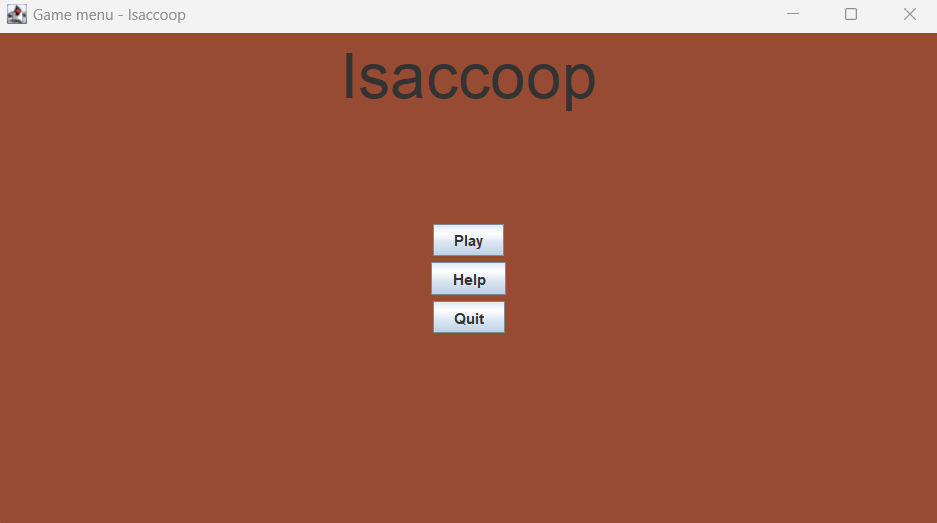
\includegraphics[width=\textwidth]{img/mainMenu.png}
\caption{Menu principale}
\label{img/standardRoom.png}
\end{figure}

\section*{Modalità di gioco}
\subsection*{Comandi del giocatore}
Esattamente come nel gioco ``The Binding of Isaac'', a cui questo applicativo si ispira liberamente, i comandi riguardanti il giocatore sono i seguenti:
\begin{itemize}
    \item \textbf{W}: Movimento verso l'alto
    \item \textbf{A}: Movimento verso sinistra
    \item \textbf{S}: Movimento verso il basso
    \item \textbf{D}: movimento verso destra
\end{itemize}
Il giocatore, per sconfiggere nemici, spara le ``onde di energia''
\begin{itemize}
    \item \textbf{↑} (Freccia SU): verso l'alto
    \item \textbf{↓} (Freccia GIU): verso il basso
    \item \textbf{←} (Freccia SINISTRA): verso sinistra
    \item \textbf{→} (Freccia DESTRA): verso destra
\end{itemize}

\subsection*{Altri comandi}
\begin{itemize}
    \item \textbf{ESC}: pausa/riprende il gioco
    \item \textbf{P}: il giocatore si sposta nella stanza successiva
    \item \textbf{N}: il giocatore si sposta nella stanza precedente
\end{itemize}

\newpage
\subsection*{Schermata di gioco}
Dopo aver cliccato il pulsante ``Play'' nel menu principale, l'utente visualizzerà la seguente schermata, caratterizzata da due sezioni principali:
\begin{itemize}
    \item \textbf{la stanza di gioco}, in alto, dove si muovono il giocatore e i nemici
    \item \textbf{la barra di stato}, in basso, dove vengono mostrate, da sinistra verso destra:
    \begin{itemize}
        \item \textit{minimappa}: mostra la struttura del livello, il numero di stanze che lo compongono e se tali stanze sono complete oppure no
        (una stanza è completa se non sono rimasti altri nemici da sconfiggere)
        \item \textit{statistiche del giocatore}: mostra alcune informazioni sullo stato del giocatore
        \item \textit{legenda}: spiega il significato dei colori utilizzati nella minimappa
    \end{itemize}
\end{itemize}

\begin{figure}[h]
\centering{}
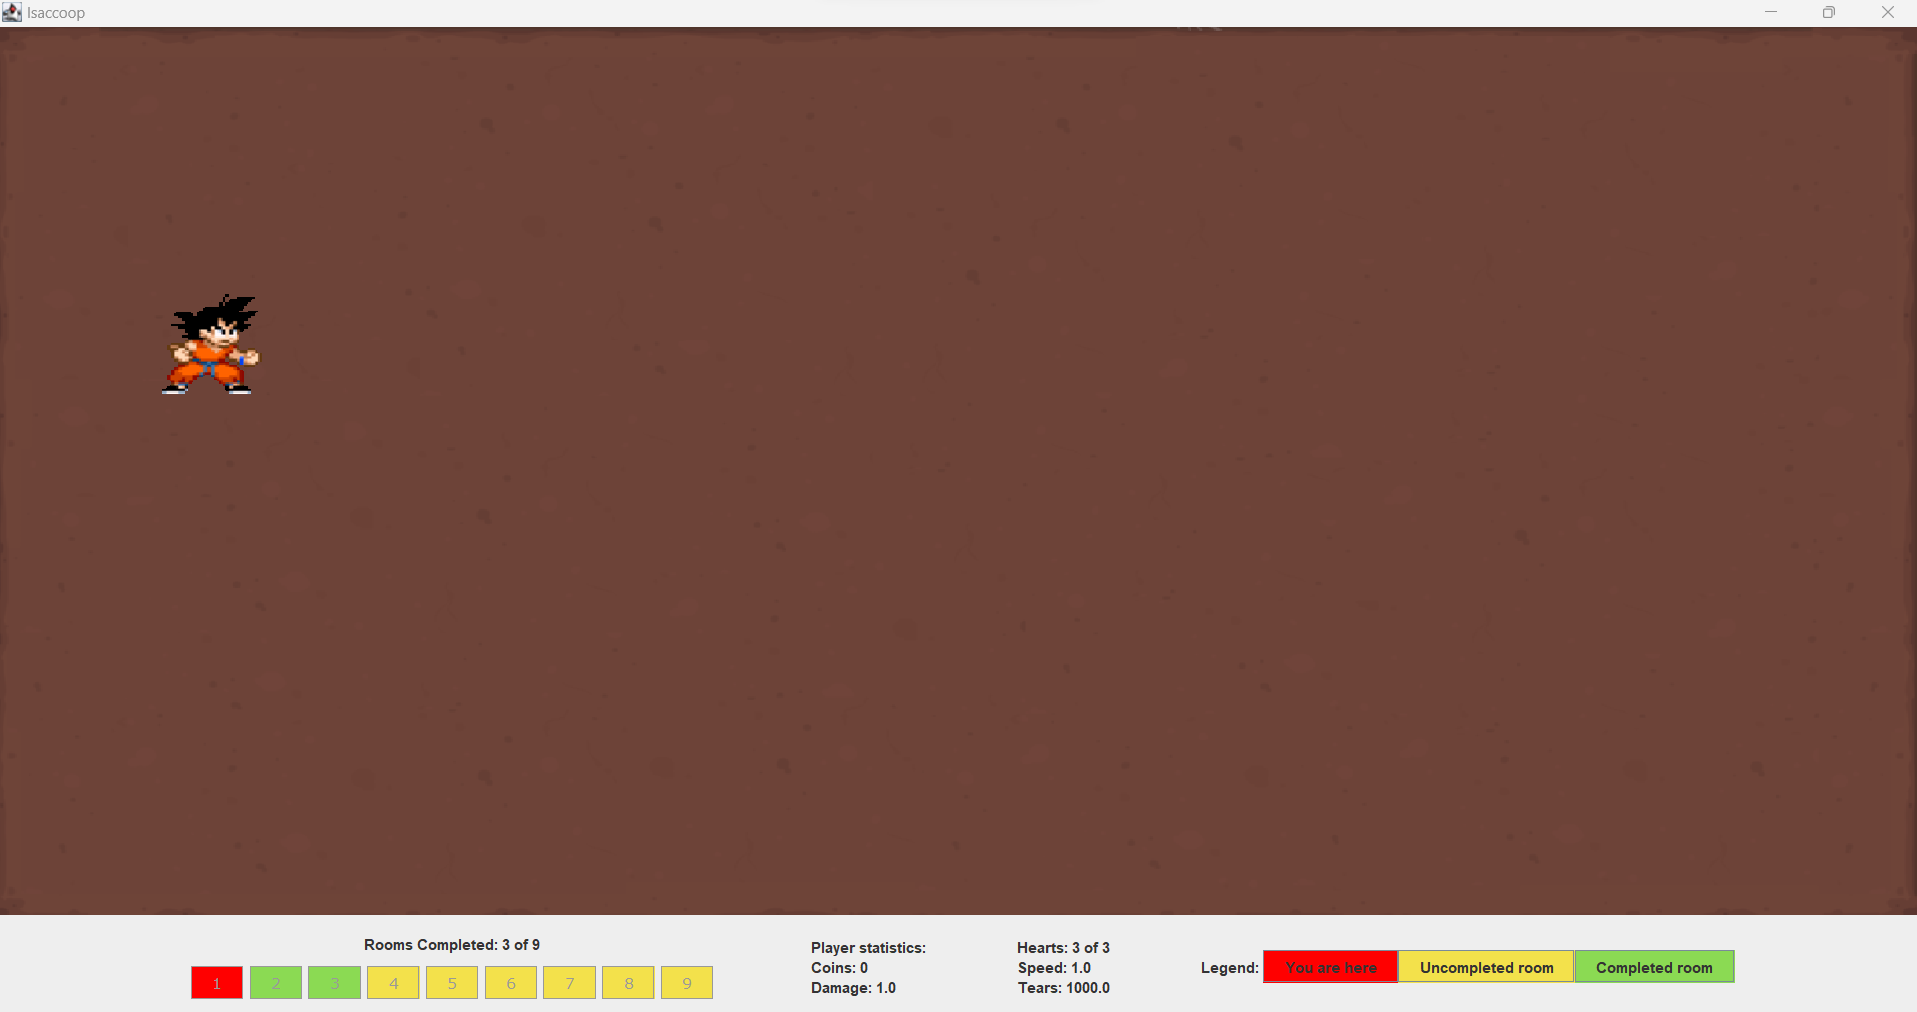
\includegraphics[width=\textwidth]{img/emptyRoom.png}
\caption{La stanza iniziale}
\label{img/emptyRoom}
\end{figure}


\newpage
Segue uno screenshot di una stanza in cui sono presenti nemici 
(elefante grigio e pianta rossa e bianca) e item (i cuori).
\begin{figure}[h]
\centering{}
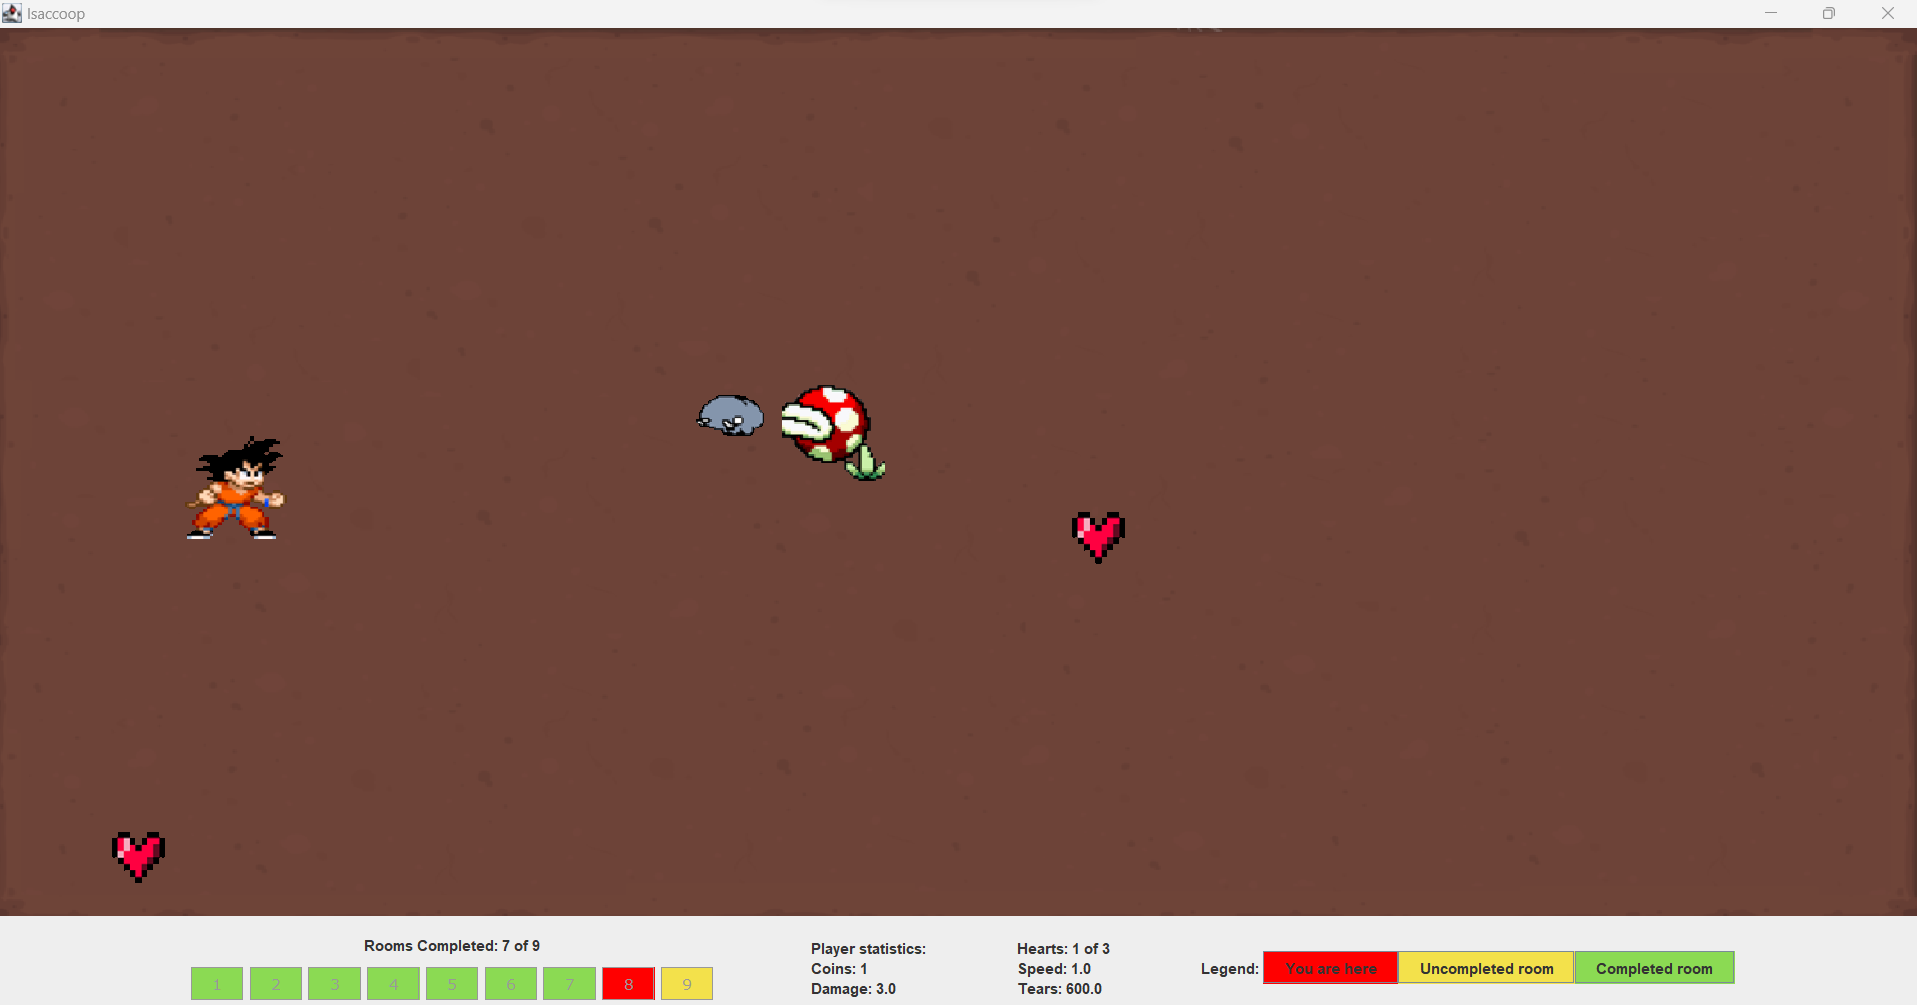
\includegraphics[width=\textwidth]{img/standardRoom.png}
\caption{Standard room con nemici e item}
\label{img/standardRoom}
\end{figure}

Se il giocatore viene colpito dai nemici e perde tutte le vite, la partita terminerà, mostrando la seguente schermata di game over.
\begin{figure}[H]
\centering{}
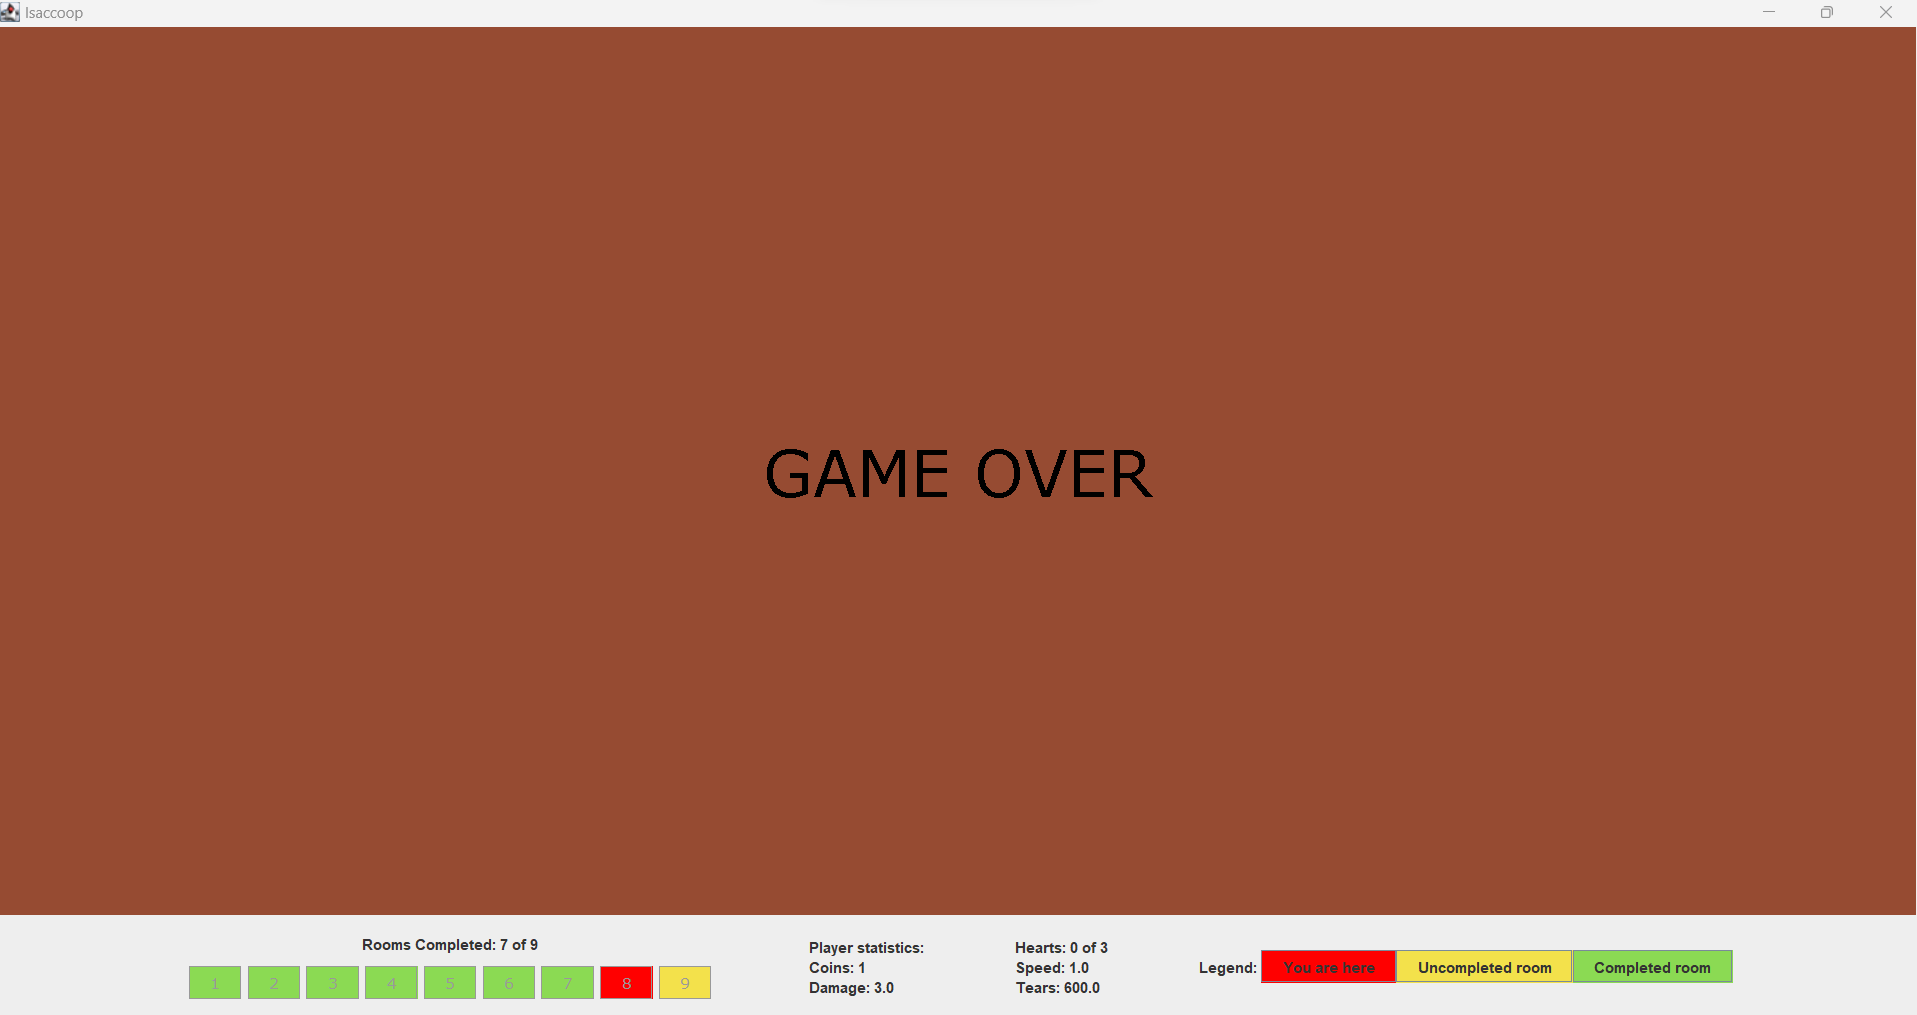
\includegraphics[width=\textwidth]{img/gameOver.png}
\caption{Schermata di game over}
\label{img/gameover}
\end{figure}

Quando il giocatore completa tutte le stanze, compresa quella del boss finale, comparirà una
schermata simile alla precedente, con la scritta ``GAME COMPLETED".

Sia nel caso di game over, sia nel caso di vittoria, per tornare al menu principale, è sufficiente cliccare 
ovunque sopra la mappa di gioco.


\chapter{Esercitazioni di laboratorio}

\section*{Esempio}

\subsection{paperon.depaperoni@studio.unibo.it}

\begin{itemize}
    \item Laboratorio 04: \url{https://virtuale.unibo.it/mod/forum/discuss.php?d=12345#p123456}
    \item Laboratorio 05: \url{https://virtuale.unibo.it/mod/forum/discuss.php?d=22222#p222222}
    \item Laboratorio 06: \url{https://virtuale.unibo.it/mod/forum/discuss.php?d=99999#p999999}
    \item Laboratorio 07: \url{https://virtuale.unibo.it/mod/forum/discuss.php?d=22222#p222222}
    \item Laboratorio 08: \url{https://virtuale.unibo.it/mod/forum/discuss.php?d=99999#p999999}
    \item Laboratorio 09: \url{https://virtuale.unibo.it/mod/forum/discuss.php?d=22222#p222222}
    \item Laboratorio 10: \url{https://virtuale.unibo.it/mod/forum/discuss.php?d=99999#p999999}
    \item Laboratorio 11: \url{https://virtuale.unibo.it/mod/forum/discuss.php?d=22222#p222222}
\end{itemize}


\bibliographystyle{alpha}
\bibliography{13-template}
\begin{itemize}
    \item Nella fase di analisi abbiamo preso spunto dalla repository del prof. Alessandro Ricci. 
    \\\url{https://github.com/pslab-unibo/oop-game-prog-patterns-2022} 
\end{itemize}
\end{document}}